\documentclass[aspectratio=169,11pt]{beamer}
\usepackage[T1]{fontenc}
\usepackage{lmodern,amsmath,amssymb,mathtools,bm,booktabs,array,graphicx,tikz}
\usetikzlibrary{arrows.meta,positioning,calc,decorations.pathreplacing,patterns}
\definecolor{ink}{HTML}{17344D}\definecolor{accent}{HTML}{087E8B}\definecolor{pale}{HTML}{EDF5F5}\definecolor{gold}{HTML}{AD6B19}
\providecommand{\dd}{\,\mathrm{d}}\providecommand{\R}{\mathbb{R}}
\providecommand{\E}{\mathbb{E}}\providecommand{\Var}{\operatorname{Var}}
\providecommand{\Cov}{\operatorname{Cov}}\providecommand{\diag}{\operatorname{diag}}
\providecommand{\norm}[1]{\left\lVert#1\right\rVert}
\providecommand{\abs}[1]{\left|#1\right|}
\usefonttheme{professionalfonts}
\setbeamercolor{normal text}{fg=black,bg=white}
\setbeamercolor{frametitle}{fg=ink,bg=white}
\setbeamercolor{title}{fg=ink}\setbeamercolor{structure}{fg=accent}
\setbeamercolor{block title}{fg=ink,bg=pale}\setbeamercolor{block body}{fg=black,bg=pale!40}
\setbeamercolor{alerted text}{fg=accent}
\setbeamerfont{frametitle}{size=\Large,series=\bfseries}
\setbeamerfont{title}{size=\LARGE,series=\bfseries}
\setbeamertemplate{navigation symbols}{}
\setbeamersize{text margin left=.7cm,text margin right=.7cm}
\setbeamertemplate{frametitle}{\vspace{.18cm}\insertframetitle\par\vspace{.1cm}{\color{accent}\hrule height .6pt}\vspace{.12cm}}
\newcommand{\notestarget}{notes.pdf}\newcommand{\noteslabel}{Notes}
\setbeamertemplate{footline}{\hspace{.7cm}\color{ink}\scriptsize Mathematical Cardiology\quad\href{\notestarget}{\noteslabel}\hfill\insertframenumber\,/\,\inserttotalframenumber\hspace{.7cm}\vspace{.18cm}}
\setbeamercovered{invisible}
\hypersetup{pdfauthor={Zan Ahmad},pdftitle={Membrane voltage and a traveling activation},pdfpagemode=UseNone}
\begin{document}
\begin{frame}[plain]\vfill
{\small\color{accent} Mathematical Cardiology \quad Lecture 4}\par\medskip
{\raggedright\hyphenpenalty=10000\exhyphenpenalty=10000\LARGE\bfseries\color{ink} Membrane voltage and a traveling activation}\par\bigskip
Zan Ahmad\par\smallskip
{\small Fall 2023}\par\vfill\end{frame}
\renewcommand{\notestarget}{notes.pdf\#note-charge-balance-gives-a-voltage-equation}
\begin{frame}[t,fragile,label=slide-three-different-observations]{Three different observations}
$V_m(t)$: one local membrane trace.\pause{}\par $t_a(x)$: an arrival time for each location.\pause{}\par ECG: a body-surface measurement of distributed activity.
\end{frame}
\renewcommand{\notestarget}{notes.pdf\#note-charge-balance-gives-a-voltage-equation}
\begin{frame}[t,fragile,label=slide-the-sign-of-membrane-voltage]{The sign of membrane voltage}
\[V_m=\phi_{\rm inside}-\phi_{\rm outside}.\]\pause{} $V_m<0$ means lower internal electric potential under this convention.
\end{frame}
\renewcommand{\notestarget}{notes.pdf\#note-charge-balance-gives-a-voltage-equation}
\begin{frame}[t,fragile,label=slide-capacitive-charge-balance]{Capacitive charge balance}
\[C_m\Delta V_m\approx h\left(I_{\rm applied}-\sum_jI_j\right).\]\pause{} Outward ionic current is positive here.\pause{}\par Dividing by $h$ gives a rate of change.
\end{frame}
\renewcommand{\notestarget}{notes.pdf\#note-charge-balance-gives-a-voltage-equation}
\begin{frame}[t,fragile,label=slide-a-current-depends-on-a-driving-difference]{A current depends on a driving difference}
\[I_j=g_j(V_m-E_j).\]\pause{} At $V_m=E_j$, this channel current is zero.\pause{}\par Positive voltage alone does not determine current direction.
\end{frame}
\renewcommand{\notestarget}{notes.pdf\#note-charge-balance-gives-a-voltage-equation}
\begin{frame}[t,fragile,label=slide-temporarily-freeze-the-conductances]{Temporarily freeze the conductances}
With $I_{\mathrm{applied}}=0$ and $g=\sum_j g_j>0$,\[\overline E=\frac{\sum_jg_jE_j}{g}.\]\pause{}\[C_m\frac{dV_m}{dt}=-g(V_m-\overline E).\]\pause{} Time scale: $C_m/g$.
\end{frame}
\renewcommand{\notestarget}{notes.pdf\#note-a-gate-equation-counts-opening-and-closing}
\begin{frame}[t,fragile,label=slide-count-gates-available-to-change]{Count gates available to change}
Closed fraction: $1-n$; open fraction: $n$.\pause{}\[\Delta n\approx h\{\alpha(1-n)-\beta n\}.\]\pause{} At equilibrium, $n=\alpha/(\alpha+\beta)$.
\end{frame}
\renewcommand{\notestarget}{notes.pdf\#note-a-gate-equation-counts-opening-and-closing}
\begin{frame}[t,fragile,label=slide-where-independence-enters]{Where independence enters}
Four identical independent gates must all be open.\pause{}\[\Pr(\text{channel open})=n\cdot n\cdot n\cdot n=n^4.\]\pause{} This is a nerve-model example, not the cardiac companion calculation.
\end{frame}
\renewcommand{\notestarget}{notes.pdf\#note-specify-the-waveform-that-is-actually-displayed}
\begin{frame}[t,fragile,label=slide-the-supplied-waveform]{The supplied waveform}
\[\begin{array}{c|rrrrr}a&0&2&12&160&220\\\hline F(a)&-85&30&15&0&-85\end{array}\]\pause{} Ages are ms; voltages are mV. Straight segments connect the listed points.
\end{frame}
\renewcommand{\notestarget}{notes.pdf\#note-specify-the-waveform-that-is-actually-displayed}
\begin{frame}[t,fragile,label=slide-interpolation-within-one-segment]{Interpolation within one segment}
\[F(a)=F_i+\frac{a-a_i}{a_{i+1}-a_i}(F_{i+1}-F_i).\]\pause{} The fraction is zero at the first endpoint and one at the second.
\end{frame}
\renewcommand{\notestarget}{notes.pdf\#note-distance-becomes-delay}
\begin{frame}[t,fragile,label=slide-a-travel-time]{A travel time}
\[t_a(x)=\frac xc.\]\pause{}\[\frac{20\ \mathrm{mm}}{0.4\ \mathrm{mm/ms}}=50\ \mathrm{ms}.\]
\end{frame}
\renewcommand{\notestarget}{notes.pdf\#note-distance-becomes-delay}
\begin{frame}[t,fragile,label=slide-evaluate-the-local-age]{Evaluate the local age}
\[a=t-t_a(x)=t-x/c.\]\pause{} At $t=80$ ms and $x=20$ mm, $a=30$ ms.\pause{}\[V_m(x,t)=F(a).\]
\end{frame}
\renewcommand{\notestarget}{notes.pdf\#note-distance-becomes-delay}
\begin{frame}[label=slide-one-shape-at-several-locations-panel-1]{Delayed local membrane-voltage traces}
\centering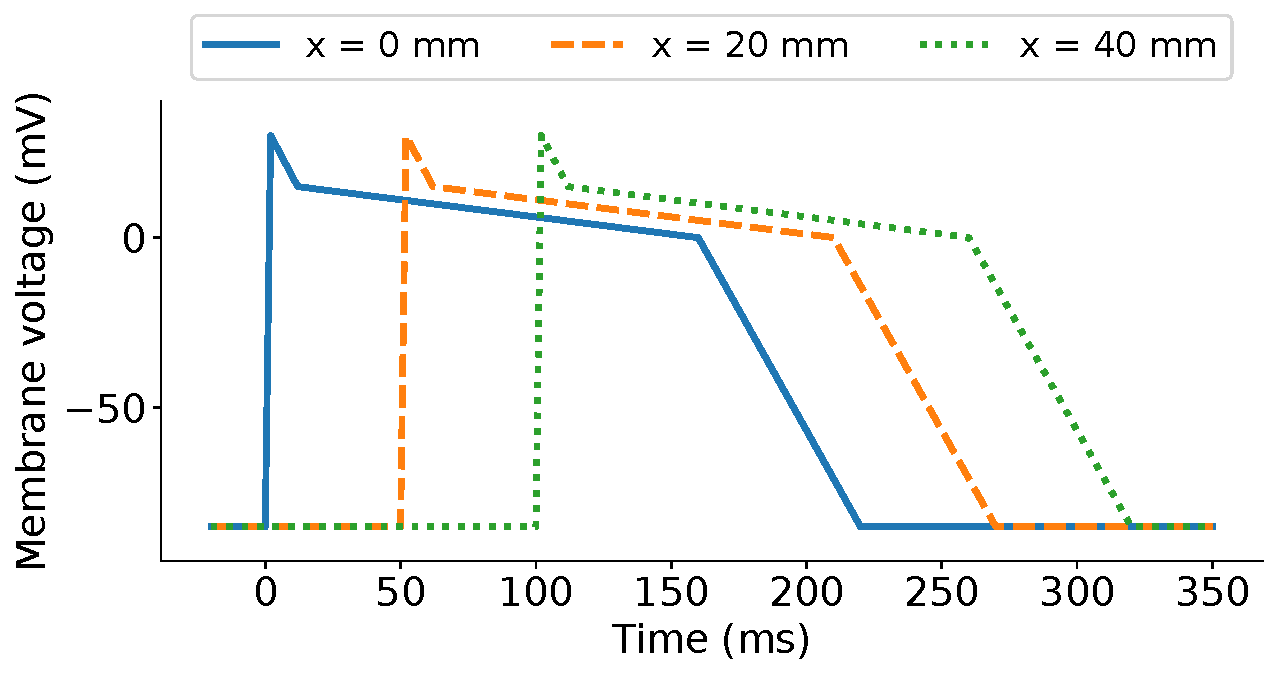
\includegraphics[width=.98\linewidth,height=.69\textheight,keepaspectratio]{presentation-figures/local-voltage-traces.pdf}\end{frame}
\renewcommand{\notestarget}{notes.pdf\#note-distance-becomes-delay}
\begin{frame}[label=slide-one-shape-at-several-locations-panel-2]{Space-time voltage at c =\allowbreak{} 0.4 mm/ms}
\centering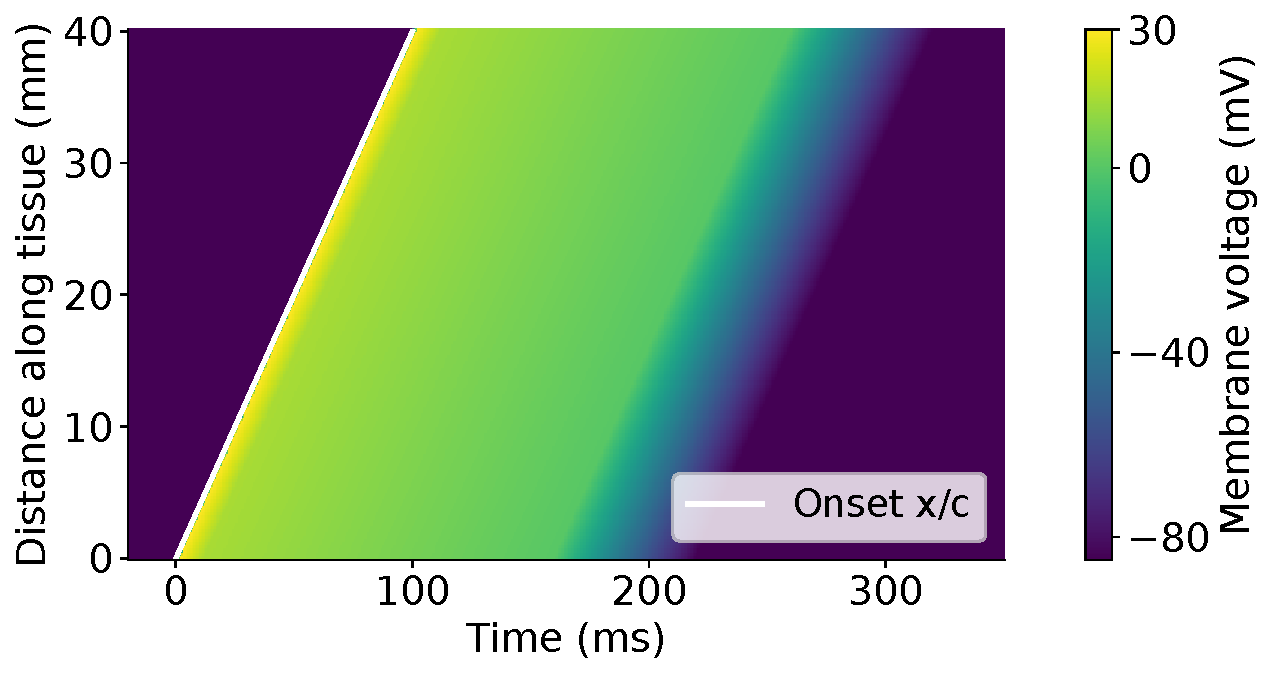
\includegraphics[width=.98\linewidth,height=.69\textheight,keepaspectratio]{presentation-figures/space-time-voltage.pdf}\end{frame}
\renewcommand{\notestarget}{notes.pdf\#note-distance-becomes-delay}
\begin{frame}[t,fragile,label=slide-one-shape-at-several-locations]{One shape at several locations}
\[V_m(x,t)=F(t-x/c).\]\pause{} Position changes delay only. The amplitude and duration remain prescribed.
\end{frame}
\renewcommand{\notestarget}{notes.pdf\#note-distance-becomes-delay}
\begin{frame}[t,fragile,label=slide-read-the-slope-on-the-actual-axes]{Read the slope on the actual axes}
For fixed local age $a_0$,\[x=c(t-a_0).\]\pause{} With time horizontal and distance vertical, the phase-line slope is $c$.
\end{frame}
\renewcommand{\notestarget}{notes.pdf\#note-a-three-dimensional-picture-of-a-one-dimensional-rule}
\begin{frame}[label=slide-the-slab-inherits-an-imposed-symmetry-panel-1]{Prescribed activation at 80 ms: c =\allowbreak{} 0.4 mm/ms}
\centering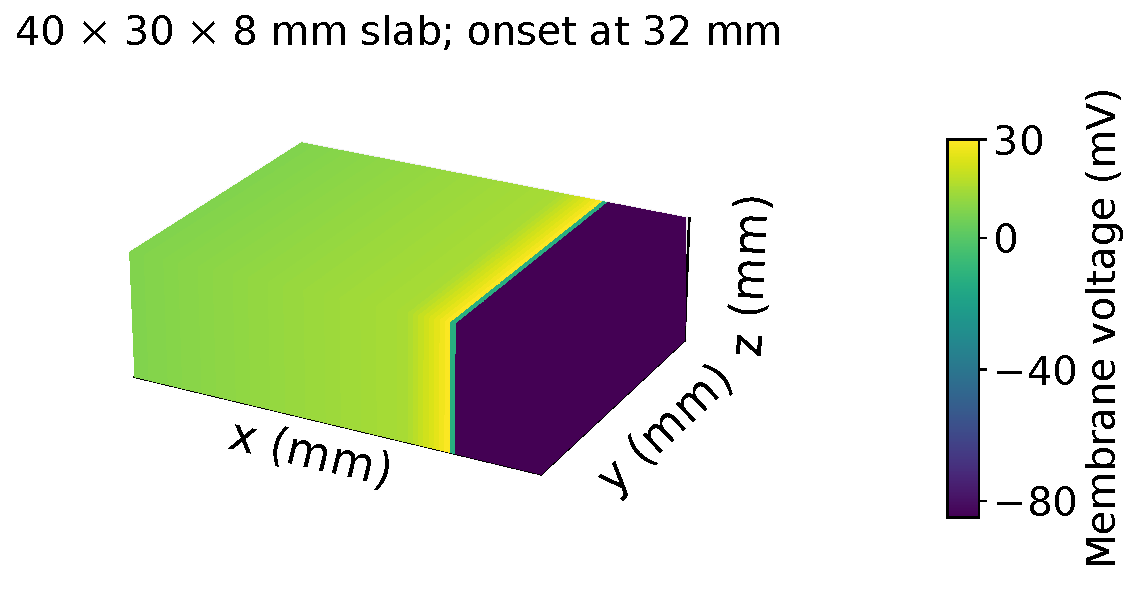
\includegraphics[width=.98\linewidth,height=.69\textheight,keepaspectratio]{presentation-figures/activation-slab-04.pdf}\end{frame}
\renewcommand{\notestarget}{notes.pdf\#note-a-three-dimensional-picture-of-a-one-dimensional-rule}
\begin{frame}[label=slide-the-slab-inherits-an-imposed-symmetry-panel-2]{Prescribed activation at 80 ms: c =\allowbreak{} 0.2 mm/ms}
\centering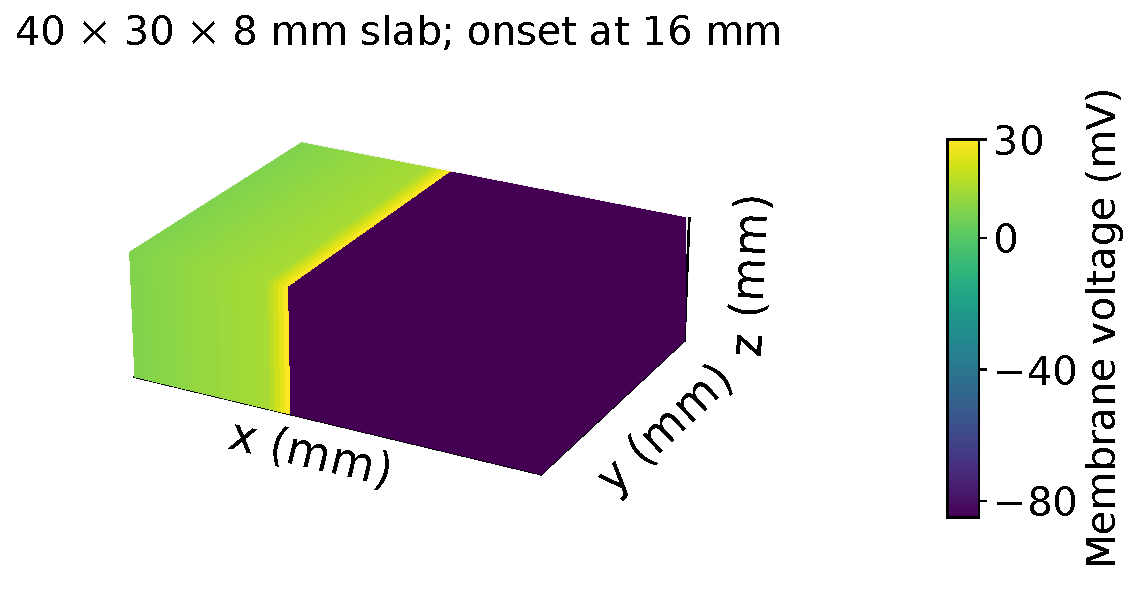
\includegraphics[width=.98\linewidth,height=.69\textheight,keepaspectratio]{presentation-figures/activation-slab-02.pdf}\end{frame}
\renewcommand{\notestarget}{notes.pdf\#note-a-three-dimensional-picture-of-a-one-dimensional-rule}
\begin{frame}[t,fragile,label=slide-the-slab-inherits-an-imposed-symmetry]{The slab inherits an imposed symmetry}
\[V_m(x,y,z,t)=F(t-x/c).\]\pause{} No $y$ or $z$ dependence is solved.\pause{}\[ct=32\ \mathrm{mm}\ \text{or}\ 16\ \mathrm{mm}\quad(t=80\ \mathrm{ms}).\]
\end{frame}
\renewcommand{\notestarget}{notes.pdf\#note-a-three-dimensional-picture-of-a-one-dimensional-rule}
\begin{frame}[t,fragile,label=slide-a-waveform-is-not-an-excitability-model]{A waveform is not an excitability model}
The construction has no stimulus, gate recovery or computed conduction speed.\pause{}\par It therefore cannot predict premature-stimulus block or reentry.\pause{}\par Multiple-location recordings can test the constant-speed assumption.
\end{frame}
\end{document}
